%%%%%%%%%%%%%%%%%%%%%%%%%%%%%%%%%%%%%%%%%%%%%%%%%%%%%%%%%%%%%%%%%%%
%%% Documento LaTeX 																						%%%
%%%%%%%%%%%%%%%%%%%%%%%%%%%%%%%%%%%%%%%%%%%%%%%%%%%%%%%%%%%%%%%%%%%
% Título:		Apéndice A
% Autor:  	Ignacio Moreno Doblas
% Fecha:  	2014-02-01
% Versión:	0.5.0
%%%%%%%%%%%%%%%%%%%%%%%%%%%%%%%%%%%%%%%%%%%%%%%%%%%%%%%%%%%%%%%%%%%%

\pagestyle{fancy}
\fancyhead[LE,RO]{\thepage}
\fancyhead[RE]{Apéndice} %
\fancyhead[LO]{\nouppercase{\rightmark}}
%\fancyhead[RE]{Parte \thepart \rightmark} %
\chapterbegin{Obtención de clave para API de Google Maps}
    
 \begin{figure}[H] \centering
    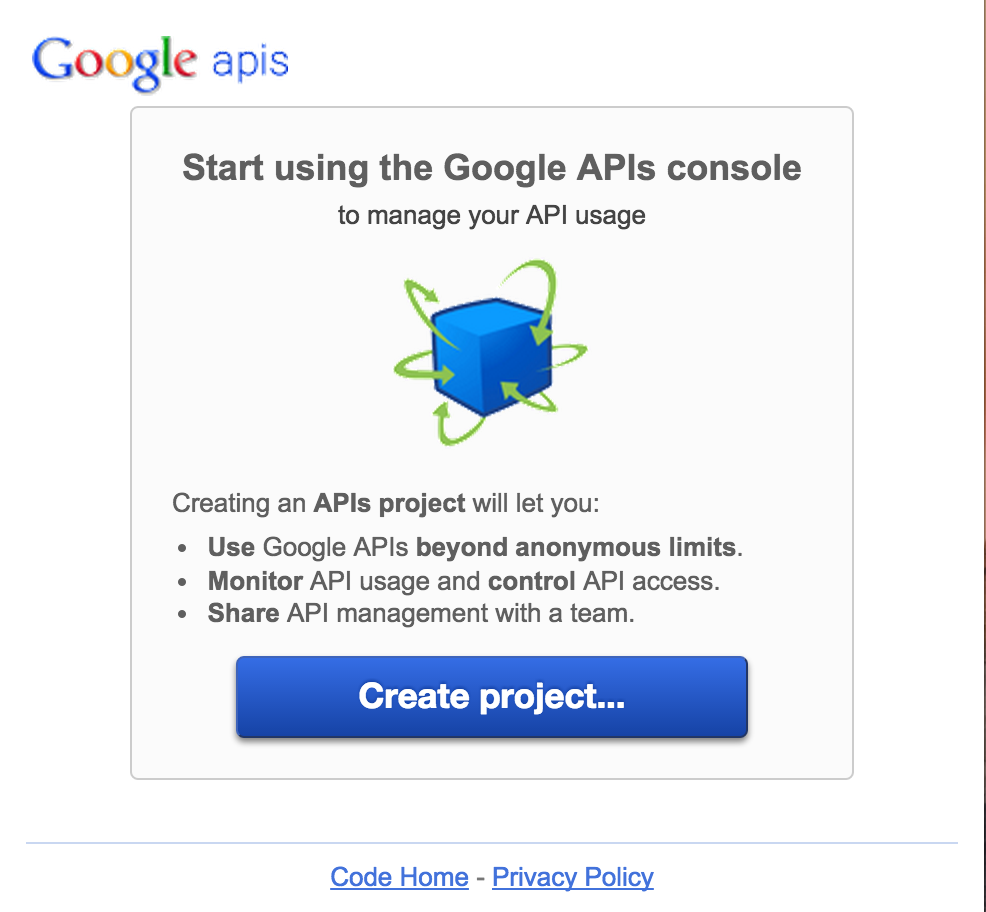
\includegraphics[height=8cm]{graphs/apicreate.png} \caption{Consola de APIs de Google sin proyectos.}\label{fig:apicreate}
\end{figure}
   
    El proceso para obtener una clave de usuaro para la API pública de Google Maps es muy parecido a obtener una clave para cualquiera del resto de APIs de Google, ya que todas pasan por la consola de APIs de Google, accesible en \mbox{\url{https://code.google.com/apis/console/}}. De ser la primera vez accediendo a la consola de APIs de Google, se muestra en pantalla la opción de crear un nuevo proyecto, tal y como se observa en la figura \ref{fig:apicreate}.

 \begin{figure}[H] \centering
    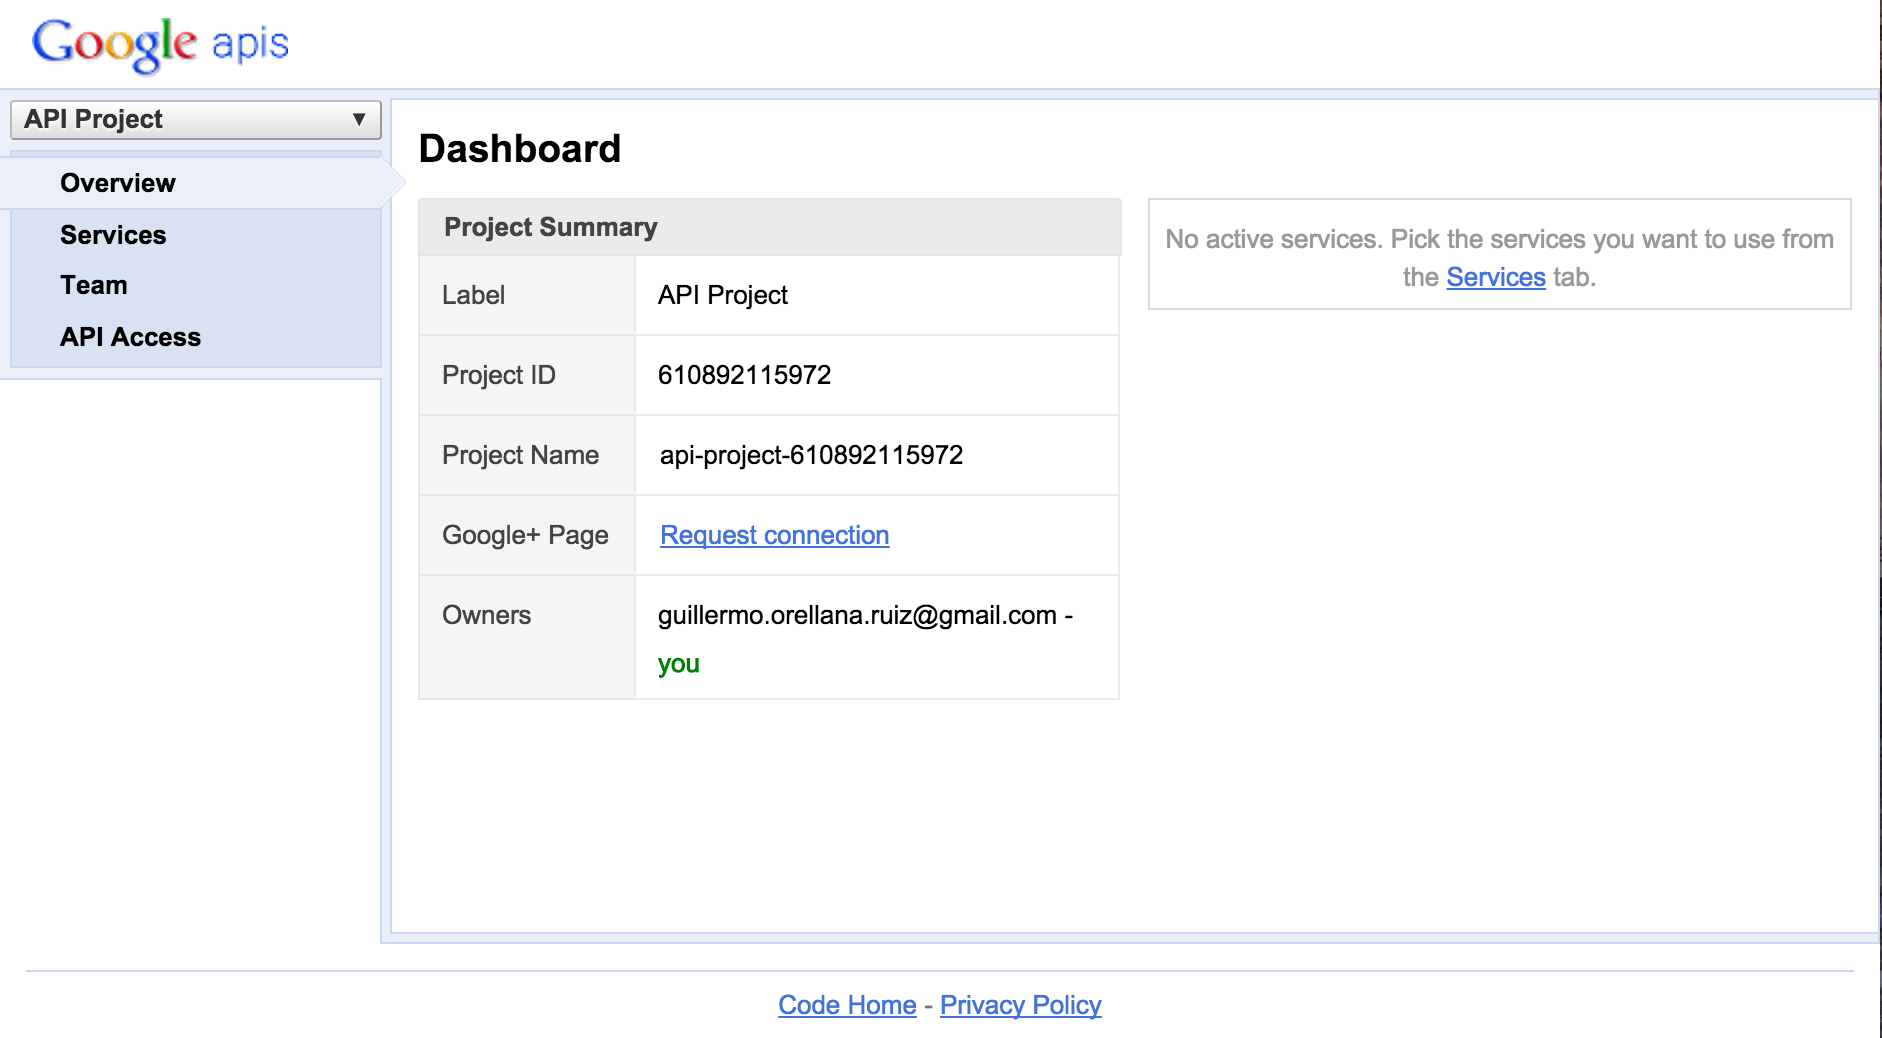
\includegraphics[width=15cm]{graphs/apidashboard.png} \caption{Proyecto \ttw{API Project} creado por defecto y en blanco.}\label{fig:apidashboard}
\end{figure}

De no haber creado ningún proyecto con anterioridad, será creado el proyecto por defecto \ttw{API Project}. Es posible configurar el nombre del proyecto a posteriori, aunque no es de importancia para el propósito de obtener una clave de API de Google Maps. El proyecto por defecto se muestra en la figura \ref{fig:apidashboard}.

 \begin{figure}[H] \centering
    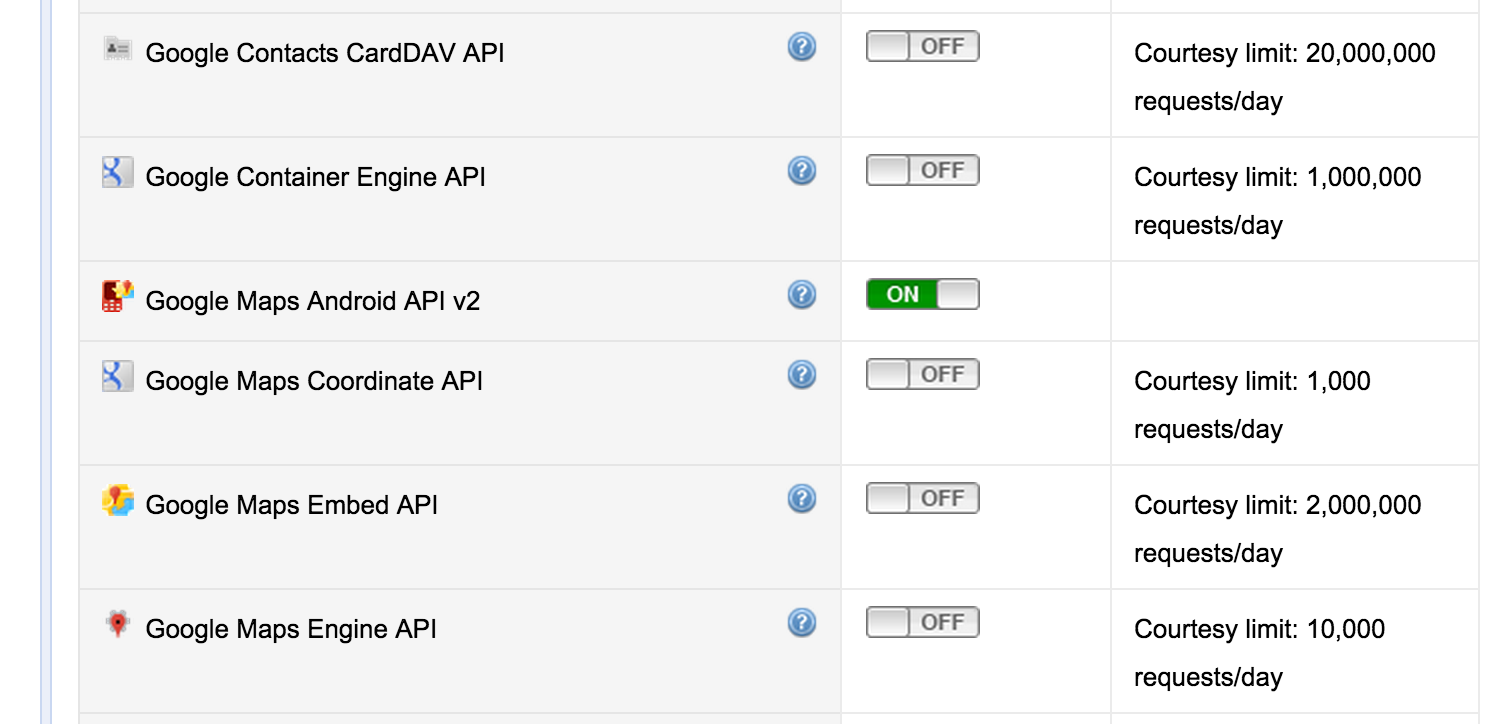
\includegraphics[width=15cm]{graphs/apion.png} \caption{Servicio \tit{Google Maps Android API v2} activado.}\label{fig:apion}
\end{figure}

Una vez en la vista de proyecto, es necesario acceder a la sección \ttw{Services}, y localizar en la lista de servicios ofrecidos por Google el llamado \tit{Google Maps Android API v2}, y activarlo. Para poder activarlo, es necesario leer y aceptar el acuerdo final de usuario, por el cual Google licencia un uso limitado de la API. Una vez que este servicio esté activado, se mostrará tal y como en la figura\ref{fig:apion}.

 \begin{figure}[H] \centering
    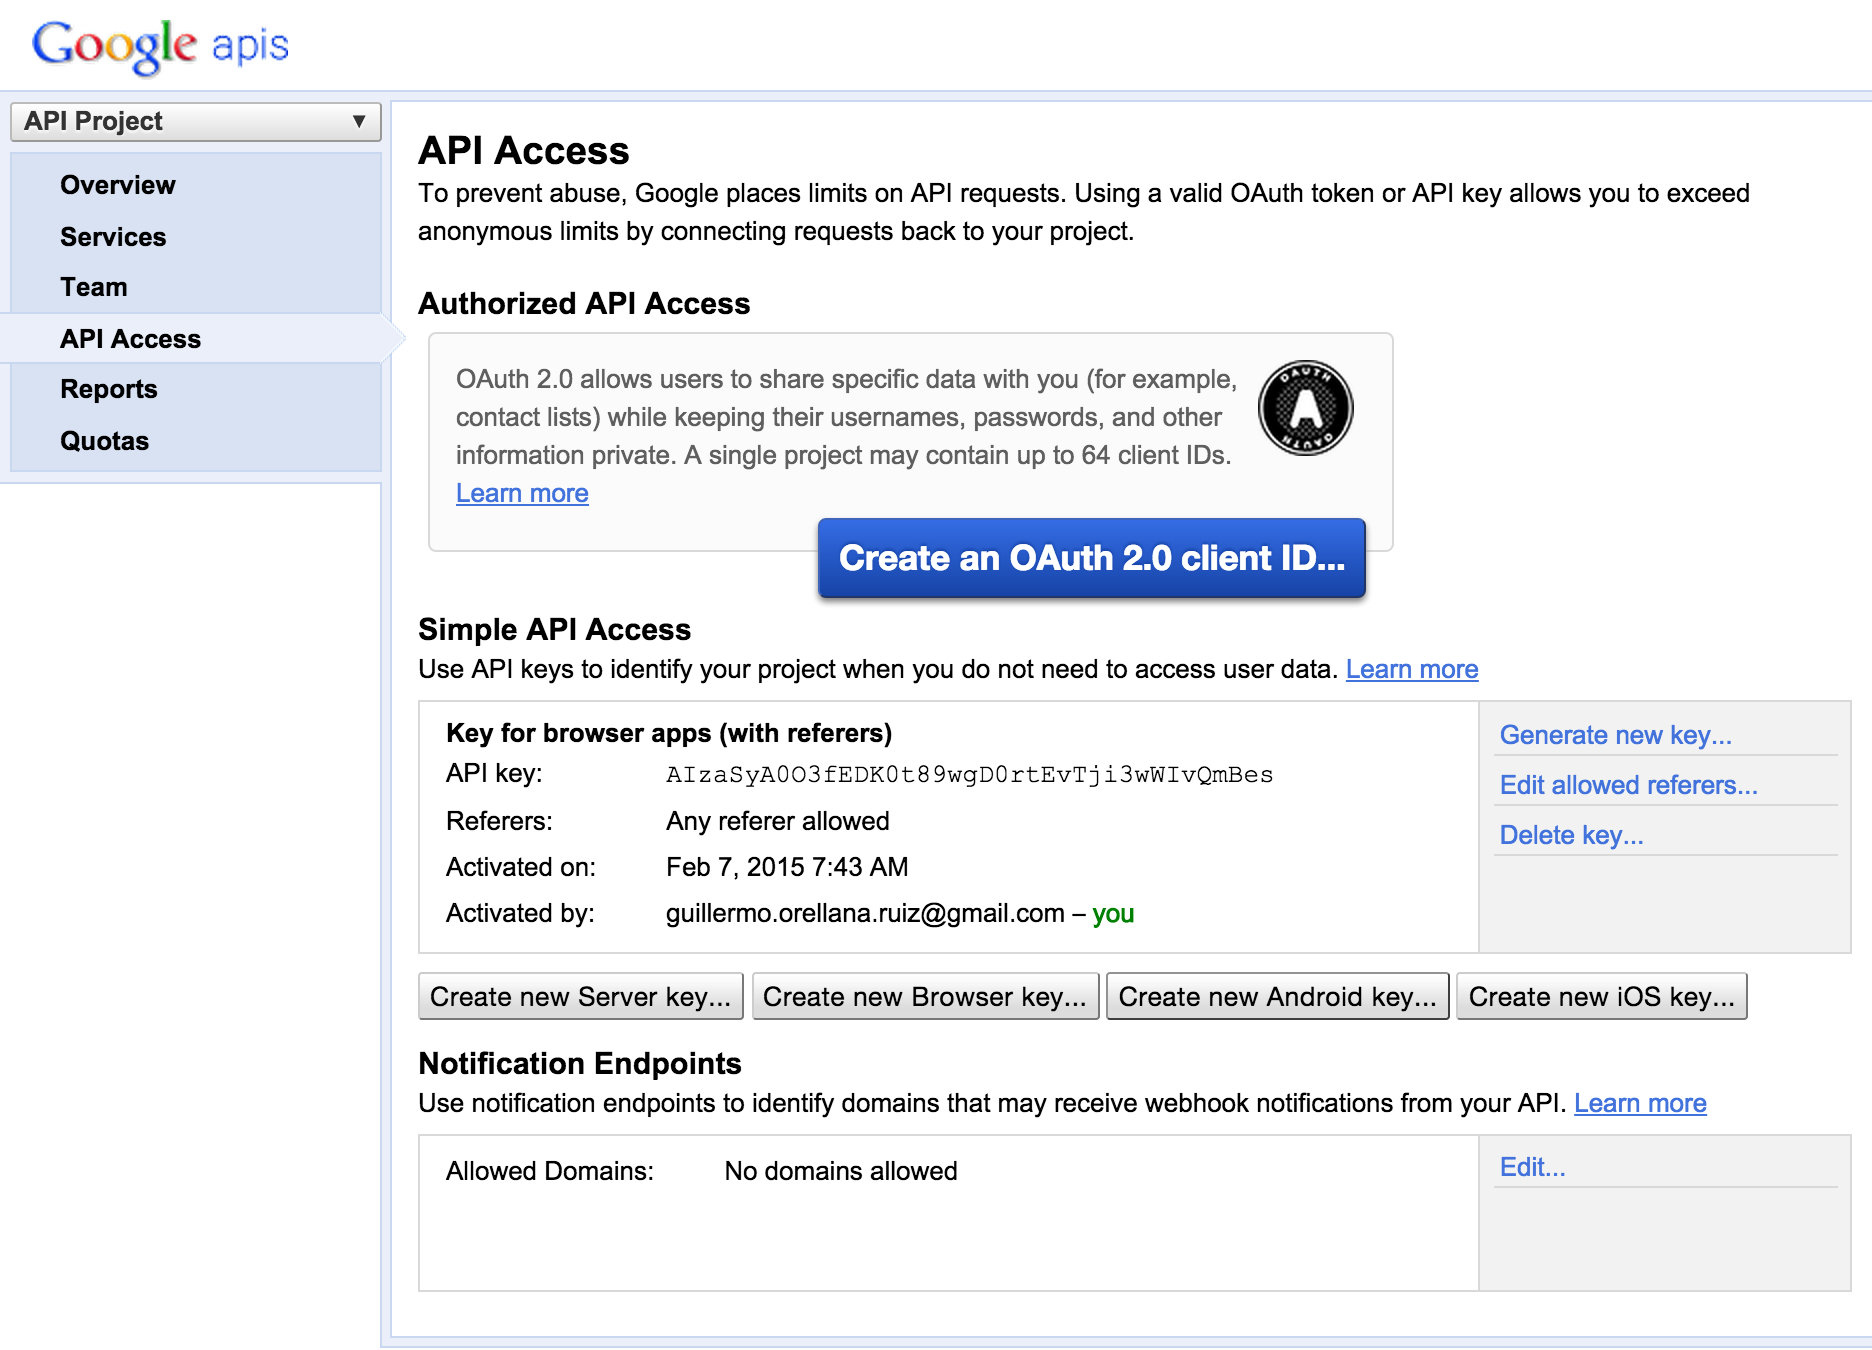
\includegraphics[width=15cm]{graphs/apikey.png} \caption{Seccion \ttw{API Access} de la consola de APIs de Google.}\label{fig:apikey}
\end{figure}

Con el servicio activado, el siguiente paso consiste en acceder a la sección \ttw{API Access}, donde se gestionan los métodos de autentificación y las claves del proyecto seleccionado. Dicha sección está representada en la figura \ref{fig:apikey}. Para continuar, es necesario presionar sobre el botón \ttw{Create new Android key...}.

 \begin{figure}[H] \centering
    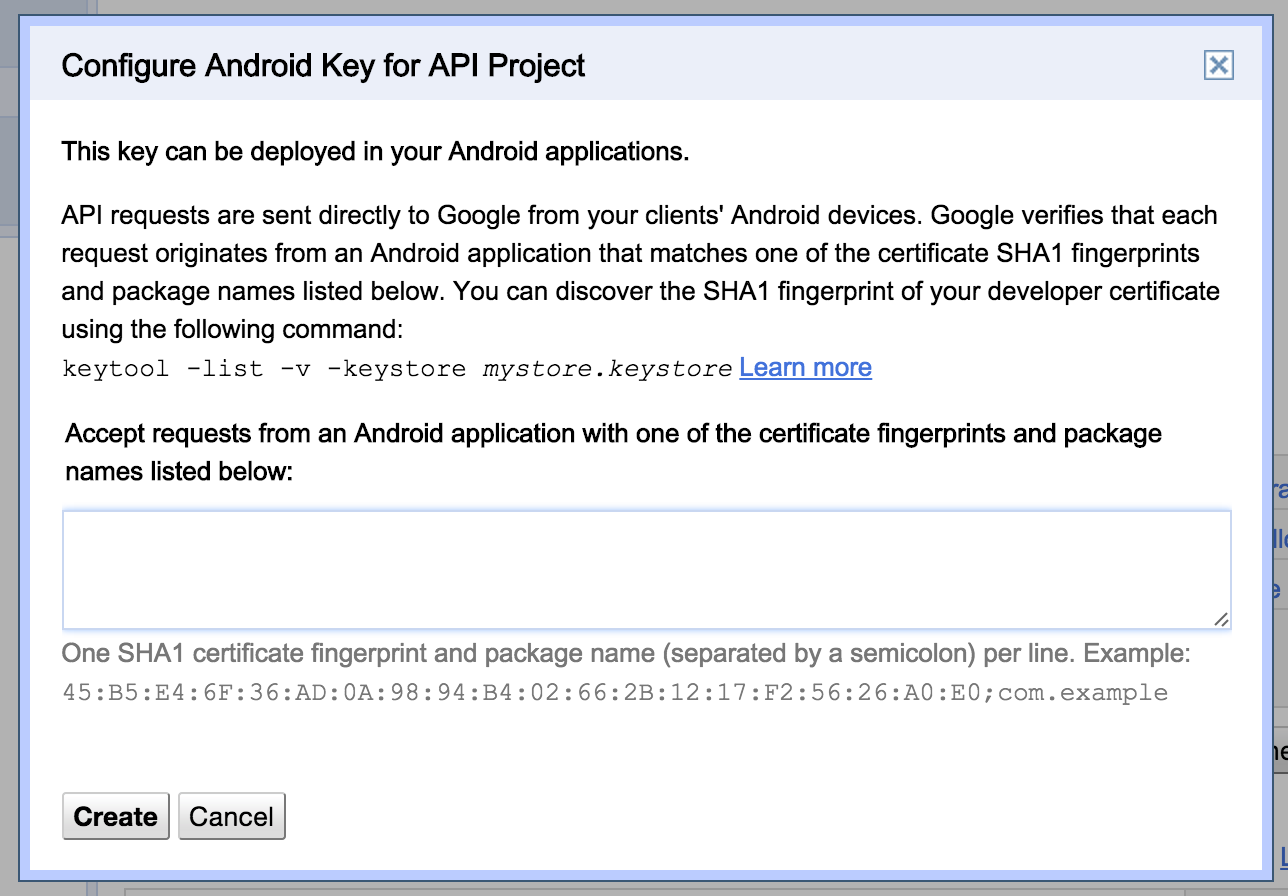
\includegraphics[width=15cm]{graphs/apikeydialog.png} \caption{Ventana de diálogo donde se introducen los datos necesarios para la clave.}\label{fig:apikeydialog}
\end{figure}

Se presenta entonces una ventana de diálogo, representada en la figura \ref{fig:apikeydialog}, en la que es necesario introducir la huella SHA-1 del certificado utilizado para firmar la aplicación, y el nombre de paquete Java de la misma. En caso de no conocer la huella SHA-1 del certificado, la misa ventana de diálogo indica la manera de obtenerla. 

 \begin{figure}[H] \centering
    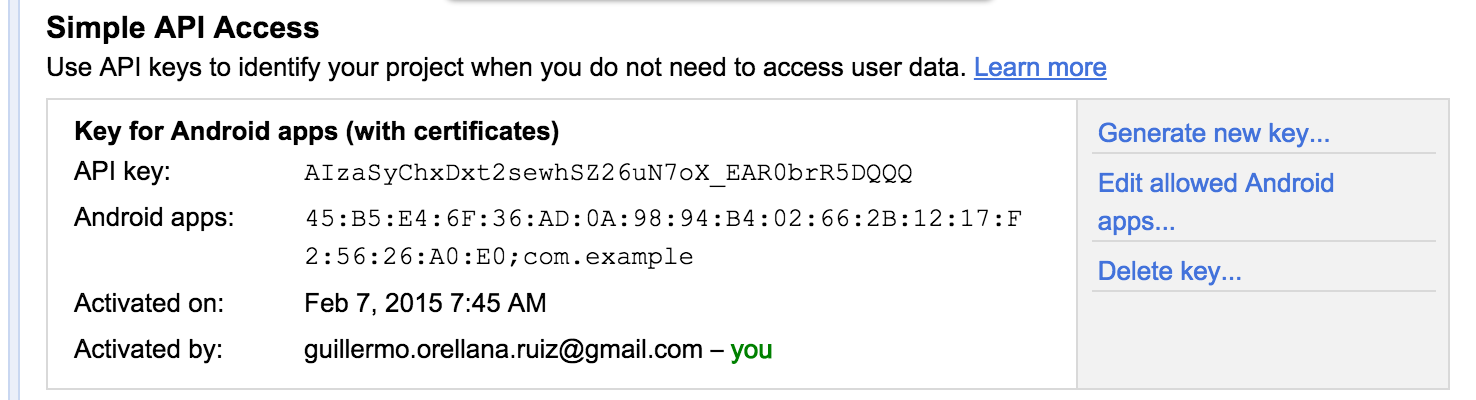
\includegraphics[width=15cm]{graphs/apikeydone.png} \caption{Sección de la consola mostrando los datos de acceso a la API.}\label{fig:apikeydone}
\end{figure}

Una vez finalizados todos los pasos, de vuelta en la sección \ttw{API Access}, habrá una nueva sección en la que estarán contenidos la clave de la API, la aplicación Android autorizada a utilizarla, la fecha de activación, y la identidad de quien la activó. Dicha sección puede ser apreciada en la figura \ref{fig:apikeydone}.

\chapterend